\chapter{Ergebnisse}
\label{chap:ergebnisse}

Nun werden, die zuvor in Kapitel \ref{chap:durchfuerung} berechneten Ergebnisse, vorgestellt.


\section{Aminosäurerest-Pseudopotential Spektren}

In einer ersten Analyse wurde die allgemeine Verteilung der \ac{APs} in Perzentile erfasst, die Ergebnisse sind in \ac{Abb} \ref{fig:quartiles_glob} und \ref{fig:quartiles_memb} dargestellt. 

\begin{figure}
\centering
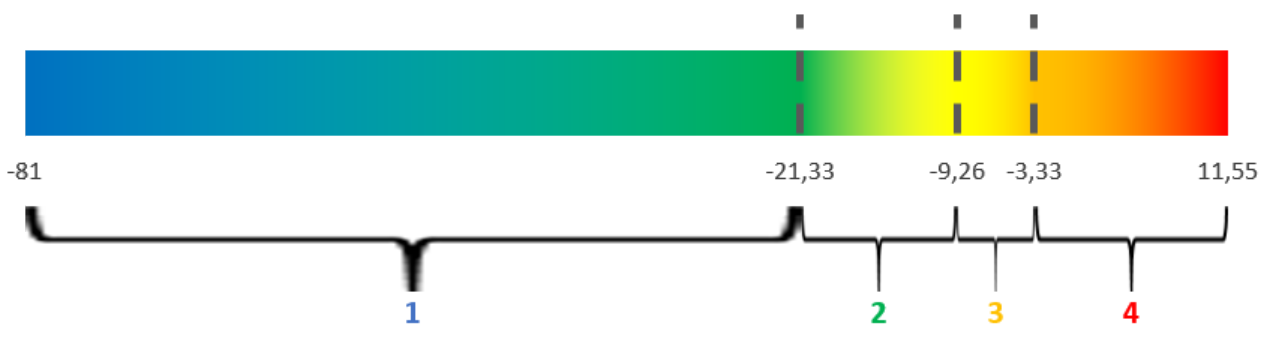
\includegraphics[width=.95\textwidth]{images/Quartil_glob.png}
\caption{Verteilung des Energiespektrums aller Energieprofile der globulären Proteine, in vier Perzentile, mit Grenzen.}
\label{fig:quartiles_glob}
\end{figure}

%new Quantile for globular:
%-81.29
%-21.53
%-9.50
%-3.44
%11.76
\begin{figure}
\centering
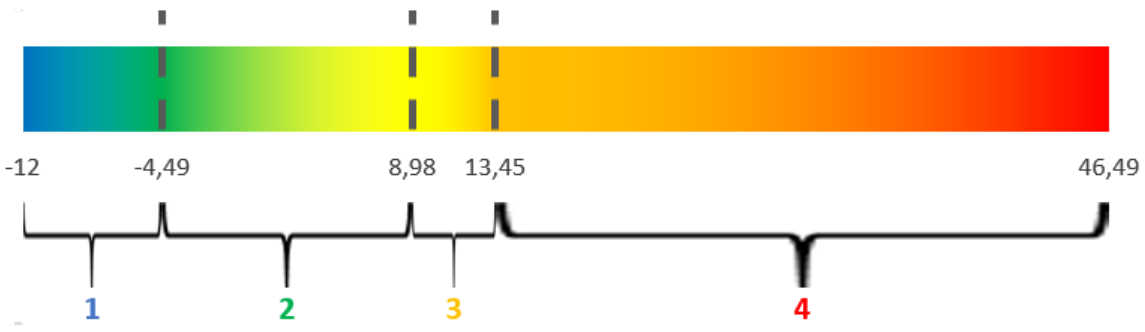
\includegraphics[width=.95\textwidth]{images/Quartil_memb.png}
\caption{Verteilung des Energiespektrums aller Energieprofile der Membran assoziierten Proteine, in vier Perzentile, mit Grenzen.}
\label{fig:quartiles_memb}
\end{figure}

%Quantile for membrane:
%-12.23
%4.49
%8.98
%13.45
%46.49

Ein dargestelltes Perzentil erfasst genau 25\% aller Energiewerte, man spricht deshalb auch von Quartilen. In \ac{Abb} \ref{fig:quartiles_glob} werden diese für alle globulären Proteine dargestellt. Das erste Quartil ist auch jenes mit dem größtem Spektrum, es reicht von -81 bis -22,21. Das zweite Quartil reicht von -21,33 bis -9,26. Das kleinste Quartil ist das dritte, es reicht von -9,26 bis -3,33 und das vierte Quartil reicht von -3,33 bis 11,55. 

In \ac{Abb} \ref{fig:quartiles_memb} werden die Quartile aller alpha helicalen Membran Proteine dargestellt, hier ist die relative Quartil Verteilung abweichend. Sodass die obere und untere Grenze sich deutlich von \ac{Abb} \ref{fig:quartiles_glob} unterscheiden, denn die untere Grenze beginnt bei -12 anstelle von -81. Die obere Grenze hingegen reicht bis +46,49 anstelle von +11,5. Demnach ist das erste Quartil von -12 bis -4,49 nicht mehr jenes mit dem größten Spektrum. Das zweite Quartil reicht von -4,49 bis 13,45, gefolgt vom drittem Quartil mit 8,98 bis 13,45.

Aufgrund der Übersichtlichkeit und durch die geringe Anzahl an alpha helicalen \ac{EP}s, befasst sich diese Arbeit hauptsächlich mit globulären Proteinen. 


\subsection{Spektrum aller Aminosäuren}

Die visualisierten Spektren der jeweiligen Aminosäuren zeigen deutliche Unterschiede auf, wie in \ac{Abb} \ref{fig:energy_ranges} zu sehen ist.

\begin{figure}
    \centering
    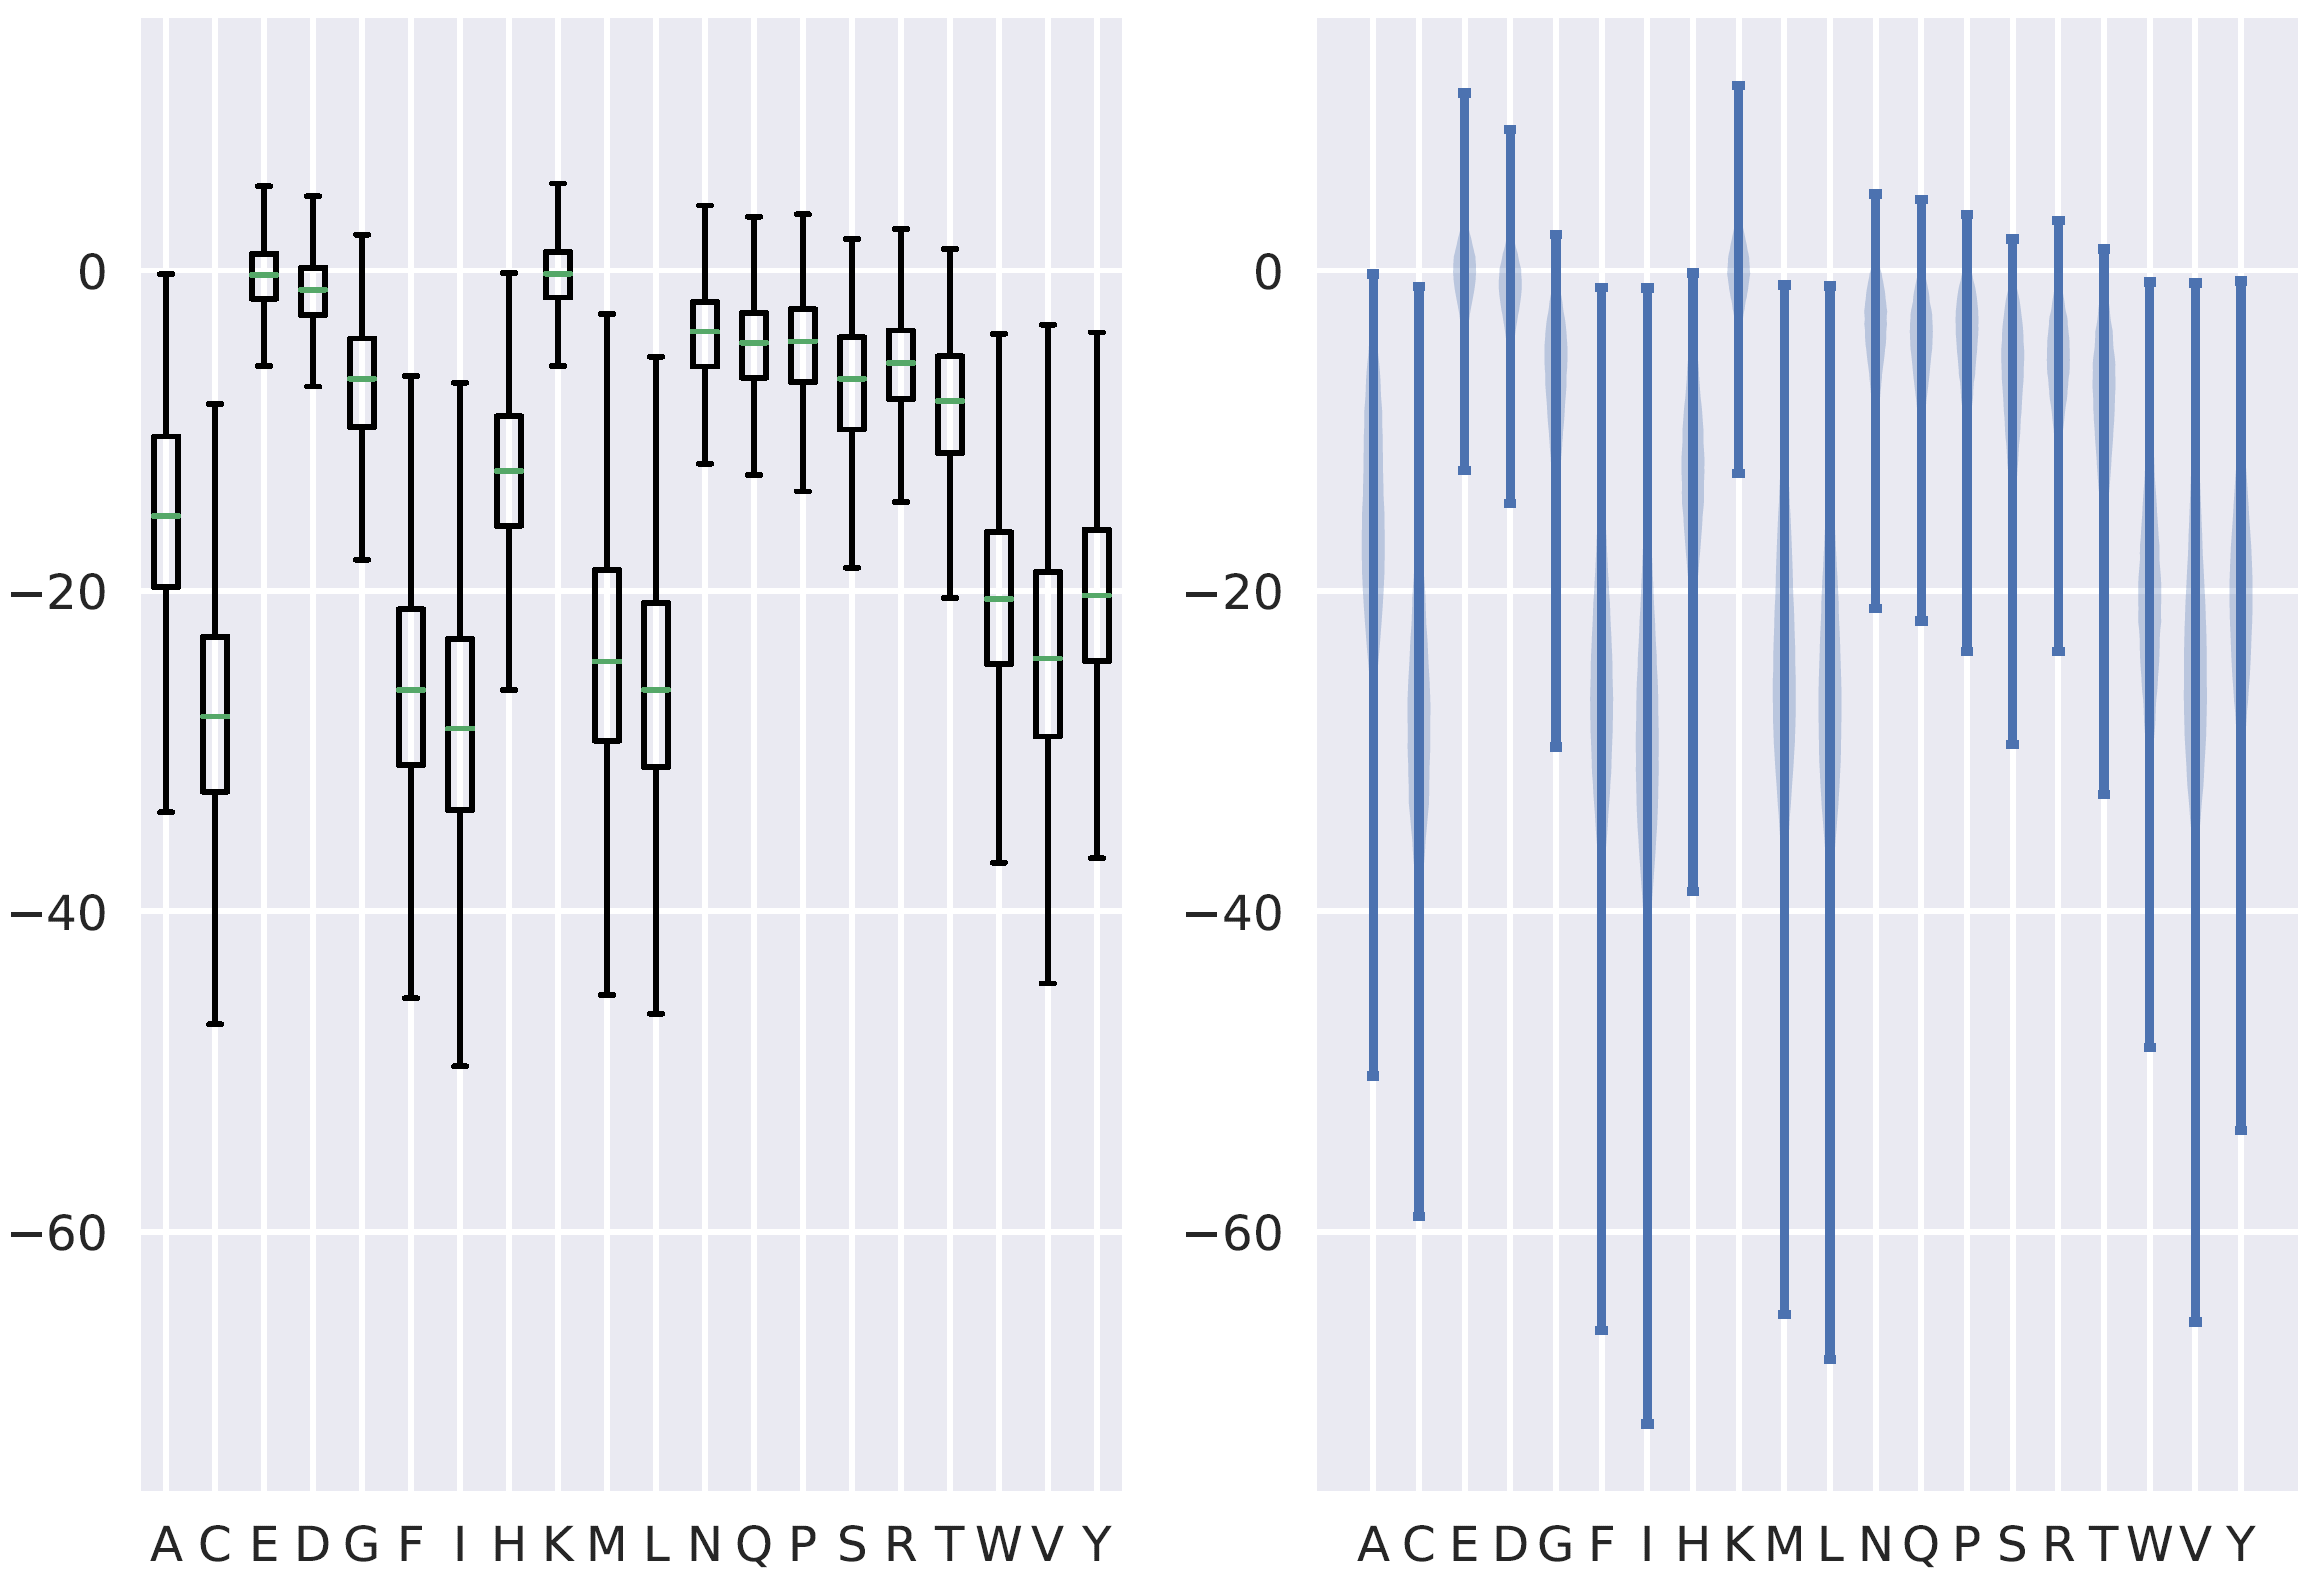
\includegraphics[width=.99\textwidth]{images/BoxPlot_energy_rages.png}
    \caption{Energien pro Aminosäure im Boxplot links und Violin Plot rechts dargestellt. Auf der Abszisse stellen die Buchstaben Abkürzungen der einzelnen Aminosäuren dar, siehe Tabelle \ref{tab:amino_table}. Auf der Ordinate sind die Energiewerte aufgetragen. Bei dem Boxplot wurden die Ausreißer mittels Grubbs-Test entfernt und die Mittelwerte mit einer grünen Markierung eingezeichnet.}
    \label{fig:energy_ranges}
\end{figure}

Zum Beispiel reicht das Spektrum der \ac{APs} von Glutaminsäure und Asparaginsäure von etwa -6 bis +6, während sich das Spektrum von Phenylalanin und Isoleuchin von -50 bis -6 bewegt. 

Zusätzlich zum Boxplot ist noch ein Violinen Plot für jede Aminosäure zu sehen. Dieser zeigt nochmals die Verteilung der Energiewerte innerhalb einer Aminosäure. Es ist so deutlich zu sehen, dass alle Werte um einen Mittelwert verteilt sind, sowie dass die Anzahl der Werte stark abflacht, sobald man sich den äußeren Bereich des jeweiligen Spektrums nähert.

Der Violinen Plot beinhaltet zudem noch alle Ausreißer, aufgrund dessen sich das Spektrum im allgemeinen länger darstellt, als es im Boxplot der Fall ist. Die Ausreißer wurden im Boxplot, mit Hilfe des Grubbs-Test \cite{Jain.2010}, herausgefiltert. 


\newpage
\subsection{Spektrum der Aminosäuren im Detail}
In diesem Abschnitt wird das Spektrum der zwei Aminosäuren, Glutaminsäure und Glycin im Detail vorgestellt. Diese beiden Aminosäuren wurden exemplarisch ausgewählt, da sich alle Aminosäurespektren ähnlich verhalten. So ist in \ac{Abb} \ref{fig:ep_as_distr} deutlich zu sehen, dass alle Energiewerte der Glutaminsäure um einen Mittelwert (-0.1) verteilt sind. Dies verhält sich sehr ähnlich für Glycin, hier sind ebenfalls alle Werte um den Mittelwert (-5.1) verteilt. Jedoch fällt auf, dass die Kurve nicht ganz symmetrisch ist, wie in der Verteilung von Energiewerten der Glutaminsäure, sondern nach links flacher abfällt. 

\begin{figure}[H]
    \subfigure[\ac{AP} Verteilung von Glutaminsäure]{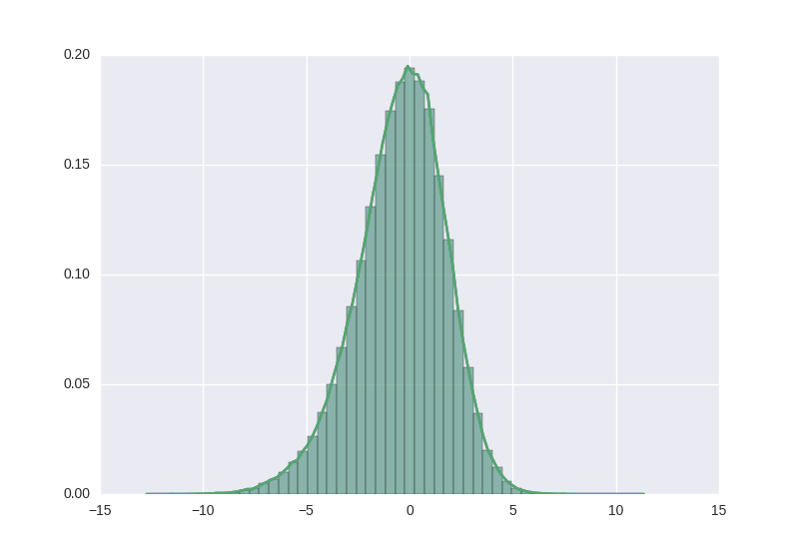
\includegraphics[width=0.49\textwidth]{images/Glutaminsaure_distr.png}}
    \subfigure[\ac{AP} Verteilung von Glycin]{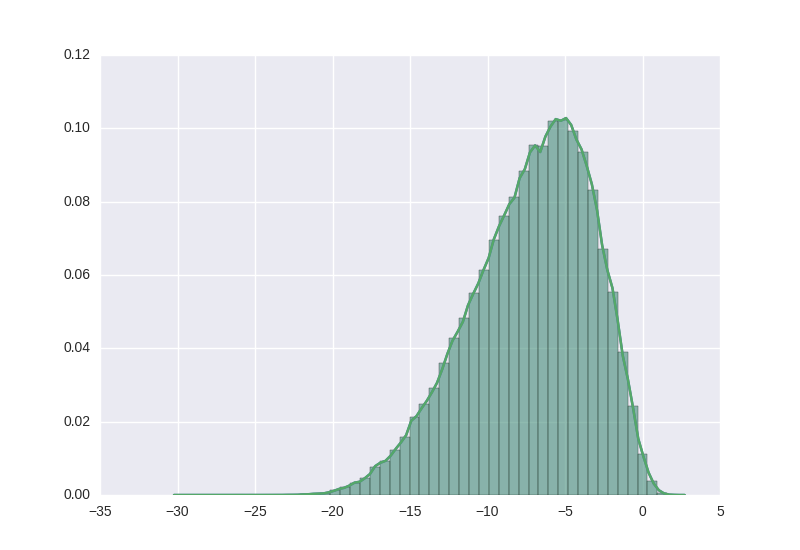
\includegraphics[width=0.49\textwidth]{images/histogramm_G.png}}
    \caption{Distribution der Energiewerte von Glutaminsäure links und Glycin rechts. Auf der Abszisse sind die Energiewerte aufgetragen und auf der Ordinate ihr relatives Vorkommen als Dezimalzahl.} 
    \label{fig:ep_as_distr}
\end{figure}

Ein Test auf Normalverteilung  hat ergeben, dass die Energiewerte nicht normalverteilt sind, da die Kurve eine zu geringe Varianz aufweist. 

Weil auch die restlichen Plots ähnlich aussehen, sind sie hier nicht dargestellt, sondern im Online Anhang dieser Arbeit zu finden.



\section{Ausgewählte Gene und SNPs}
Die in Kapitel \ref{sec:clinvar_filter} ausgesuchten \ac{SNP}s sind nun hier in Tabelle \ref{tab:expert_snps} und \ref{tab:multiple_subs_snps} dargestellt:

\begin{table}[H]
    \centering
    \caption{Tabelle aller Gene des \emph{expert panels} mit mindestens 10 pathogenen \ac{SNP}s. Die verwendeten Gene sind grün markiert.}
    \label{tab:expert_snps}
    \resizebox{\linewidth}{!}{%
    \begin{tabular}{llllllll}
    \hline
    \multicolumn{1}{|l|}{Name} & \multicolumn{1}{l|}{Template} & \multicolumn{1}{l|}{Länge} & \multicolumn{1}{l|}{Coverage} & \multicolumn{1}{l|}{Identität} & \multicolumn{1}{l|}{QMEAN} & \multicolumn{1}{l|}{SNPs} & \multicolumn{1}{l|}{Assoziierung} \\ \hline
    \rowcolor[HTML]{9AFF99} 
    MSH2 & 3thw.1.A & 934 & 98,40\% & 100\% & -2,05 & 33 & globulär \\ \hline
    \multicolumn{1}{|l}{BRCA1} & 1jm7.1.A & 1863 & 5,50\% & 100\% & -0,13 & 24 & \multicolumn{1}{l|}{globulär} \\
    \multicolumn{1}{|l}{} & 4y18.1.A &  & 11,40\% &  & -2,18 &  & \multicolumn{1}{l|}{} \\ \hline
    BRCA2 & 1miu.1.B & 3418 & 21\% & 75,48\% & -5,05 & 10 & globulär \\
    \rowcolor[HTML]{9AFF99} 
    CFTR & 5uak.1.A & 1480 & 96,70\% & 100\% & -4,51 & 44 & membran \\
    MYH7 & 5tby.1.A & 1935 & 49,50\% & 100\% & -4,8 & 32 & globulär \\ \hline
    \multicolumn{1}{|l}{MLH1} & 4p7a.1.A & 756 & 44\% & 100\% & -0,73 & 65 & \multicolumn{1}{l|}{globulär} \\
    \multicolumn{1}{|l}{} & 3rbn.1.A &  & 34,90\% & 100\% & -1,29 &  & \multicolumn{1}{l|}{} \\ \hline
    \end{tabular}}
\end{table}

Wie in der ersten Tabelle zu sehen ist, ist die größte Coverage bei \texttt{MSH2} mit 98,4\%, gefolgt von \texttt{CFTR} mit 96,7\%. Die Sequenzidentität beträgt bei beiden 100\%. Bei fast allen Sequenzen wurden mehrere Templates gefunden, doch die Meisten weisen eine sehr niedrige Coverage auf, sodass sie hier nicht dargestellt sind. Bei \texttt{MLH1} wurden zwei Templates gefunden, welche 44\% und 34,9\% der Sequenz abdecken. Bei \texttt{BRCA1} wurden ebenfalls mehrere Templates gefunden, sodass hier eine Coverage von 11,4\% und 5,5\% vorliegt. \texttt{BRCA2} hat eine Coverage von 21\% bei 75,48\% Sequenzidentität. Letztendlich wurden nur die \ac{SNP}s von \texttt{MSH2} und \texttt{CFTR} in dieser Arbeit verwendet.

In einem zweiten Durchgang wurden auch alle Proteine mit ihren SNPs aus Tabelle \ref{tab:multiple_subs_snps} mittels Swissmodel strukturell modelliert. Hierbei zeigte \texttt{ABCA4} die höchste Coverage mit 98,90\% und Sequenzidentität von 51,97\%. Betrachtet man Coverage und Sequenzidentität in Abhängigkeit, so weist \texttt{ACADM} die höchste Coverage mit 91,7\% und \texttt{SLC2A1} die zweit höchste mit 90,7\% auf. Die Sequenzidentität beträgt bei \texttt{ACADM} 100\% und bei \texttt{SLC2A1} 99,59\%, dies bedeutet, dass bei \texttt{SLC2A1}, im Vergleich zur Swissmodel Referenz, alle bis auf eine Aminosäure übereinstimmen.

Zusätzlich wurden noch \texttt{KCNQ1}, \texttt{KCNH2} und \texttt{SDHB} in den Datnesatz aufgenommen. Die restlichen Gene wurden nicht in den Datensatz aufgenommen.

\begin{table}[]
    \centering
    \caption{Tabelle aller Gene der ClinVar Datenbank, mit mindestens 6 pathogenen SNPs und multiplen Autoren, ohne Widerspruch. Dunkles grün steht für eine gute Coverage und Sequenzidentität, hellgrün zeigt die Gene, welche keine so hohe Coverage aufweisen, aber dennoch in den Datensatz aufgenommen wurden.}
    \label{tab:multiple_subs_snps}
    \resizebox{\linewidth}{!}{%
    \begin{tabular}{llllllll}
    \hline
    \multicolumn{1}{|l|}{Name} & \multicolumn{1}{l|}{Template} & \multicolumn{1}{l|}{Länge} & \multicolumn{1}{l|}{Coverage} & \multicolumn{1}{l|}{Identität} & \multicolumn{1}{l|}{QMEAN} & \multicolumn{1}{l|}{SNPs} & \multicolumn{1}{l|}{Assoziierung} \\ \hline
    MFN2 & 5gom.1.A & 757 & 51,30\% & 71.21\% & -1,32 & 13 & globulär \\
    \rowcolor[HTML]{CBFFCB} 
    SDHB & 1zoy.1.B & 280 & 85,70\% & 97.54\% & -0,88 & 10 & Membran \\
    MUTYH & 3n5n.2.A & 535 & 51,40\% & 100\% & -1,8 & 14 & globulär \\
    ALPL & 1zef.1.A & 524 & 90\% & 58,58\% & -2,04 & 8 & globulär \\
    \rowcolor[HTML]{9AFF99} 
    SLC2A1 & 4pyp.1.A & 492 & 90,70\% & 99,59\% & -4,75 & 8 & Membran \\
    \rowcolor[HTML]{9AFF99} 
    ACADM & 1ege.1.B & 421 & 91,70\% & 100\% & -1,23 & 11 & globulär \\
    LMNA & 1ufg.1.A & 572 & 22,70\% & 96,18\% & -4,66 & 21 & globulär \\
    ABCA4 & 5xjy.1.A & 2273 & 98,90\% & 51,97\% & -6,57 & 22 & Membran \\
    TNNT2 & 1j1d.2.B & 295 & 25,10\% & 99,03\% & 0,87 & 10 & globulär \\
    COL9A2 & 5ctd.1.B & 689 & 6,30\% & 86,67\% & 0,41 & 6 & globulär \\
    STIL & 4yyp.1.B & 1288 & 100\% & 2\% & -0,03 & 6 & globulär \\
    AGL & 5d06.2.A & 1532 & 43,09\% & 97,30\% & -4,43 & 8 & globulär \\
    \rowcolor[HTML]{CBFFCB} 
    KCNQ1 & 5vms.1.A & 676 & 68,50\% & 83,30\% & -5,87 & 10 & Membran \\
    \rowcolor[HTML]{CBFFCB} 
    KCNH2 & 5va2.1.A & 1159 & 74,20\% & 96,56\% & -5,38 & 6 & Membran \\
    PMS2 & 1h7s.1.A & 862 & 39\% & 100\% & 0,25 & 6 & globulär
    \end{tabular}}
\end{table}



\section{SNPs in Energieprofilen}

Die in Kapitel \ref{sec:plot_eps} berechneten Plots sind nun hier dargestellt, in \ac{Abb} \ref{fig:comp_plot_MSH2} ist ein beispielhafter Ausschnitt aus dem globulären Protein \texttt{MSH2} dargestellt. Die Abszisse gibt die Positionen der fortlaufenden Aminosäuren an, auf der Ordinate befinden sich die Energiewerte. Zu sehen ist im oberen Bild die Referenzsequenz in Blau und die Sequenz mit dem \ac{SNP} Ile169Val in Rot. Die mutierte Sequenz ist nur sichtbar, wenn sie sich von der Referenzsequenz unterscheidet, zum besseren Überblick ist zusätzlich noch die Differenz der beiden Sequenzen als die grüne Linie aufgetragen. Die gelbe Markierung zeigt die Position der \ac{SNP}s. 

\begin{figure}
    \centering
    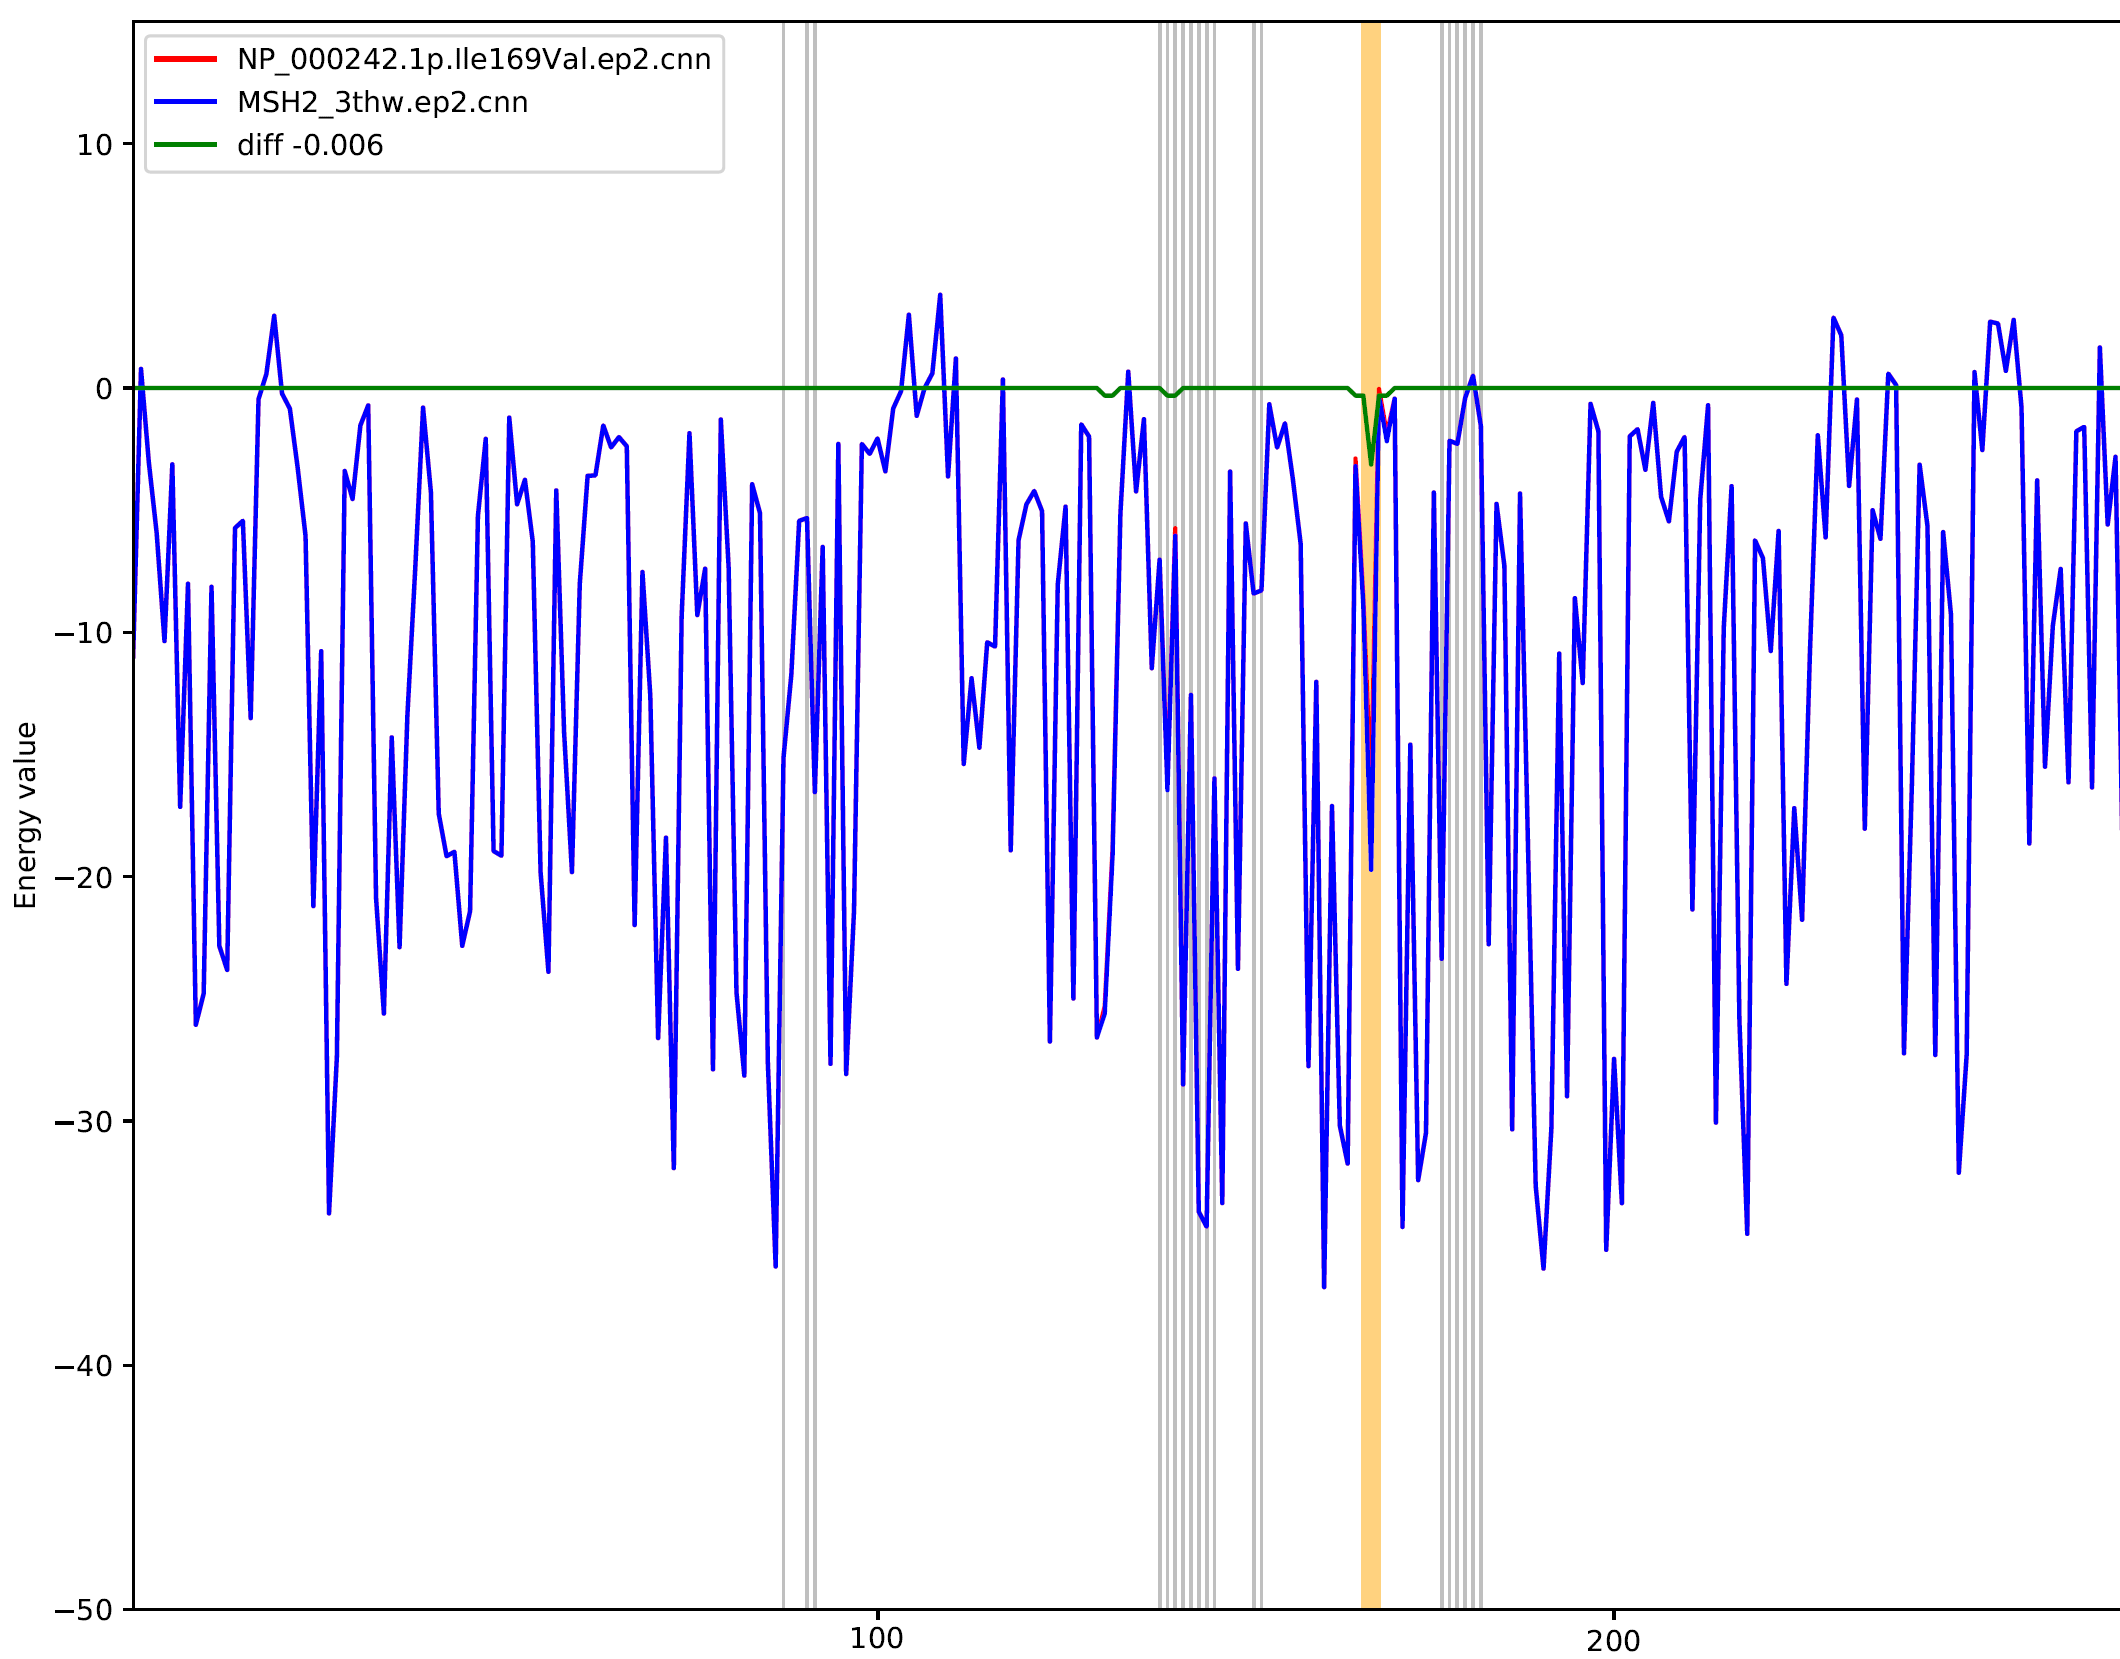
\includegraphics[width=.90\textwidth]{images/comp_plot_Ile169Val.png}
    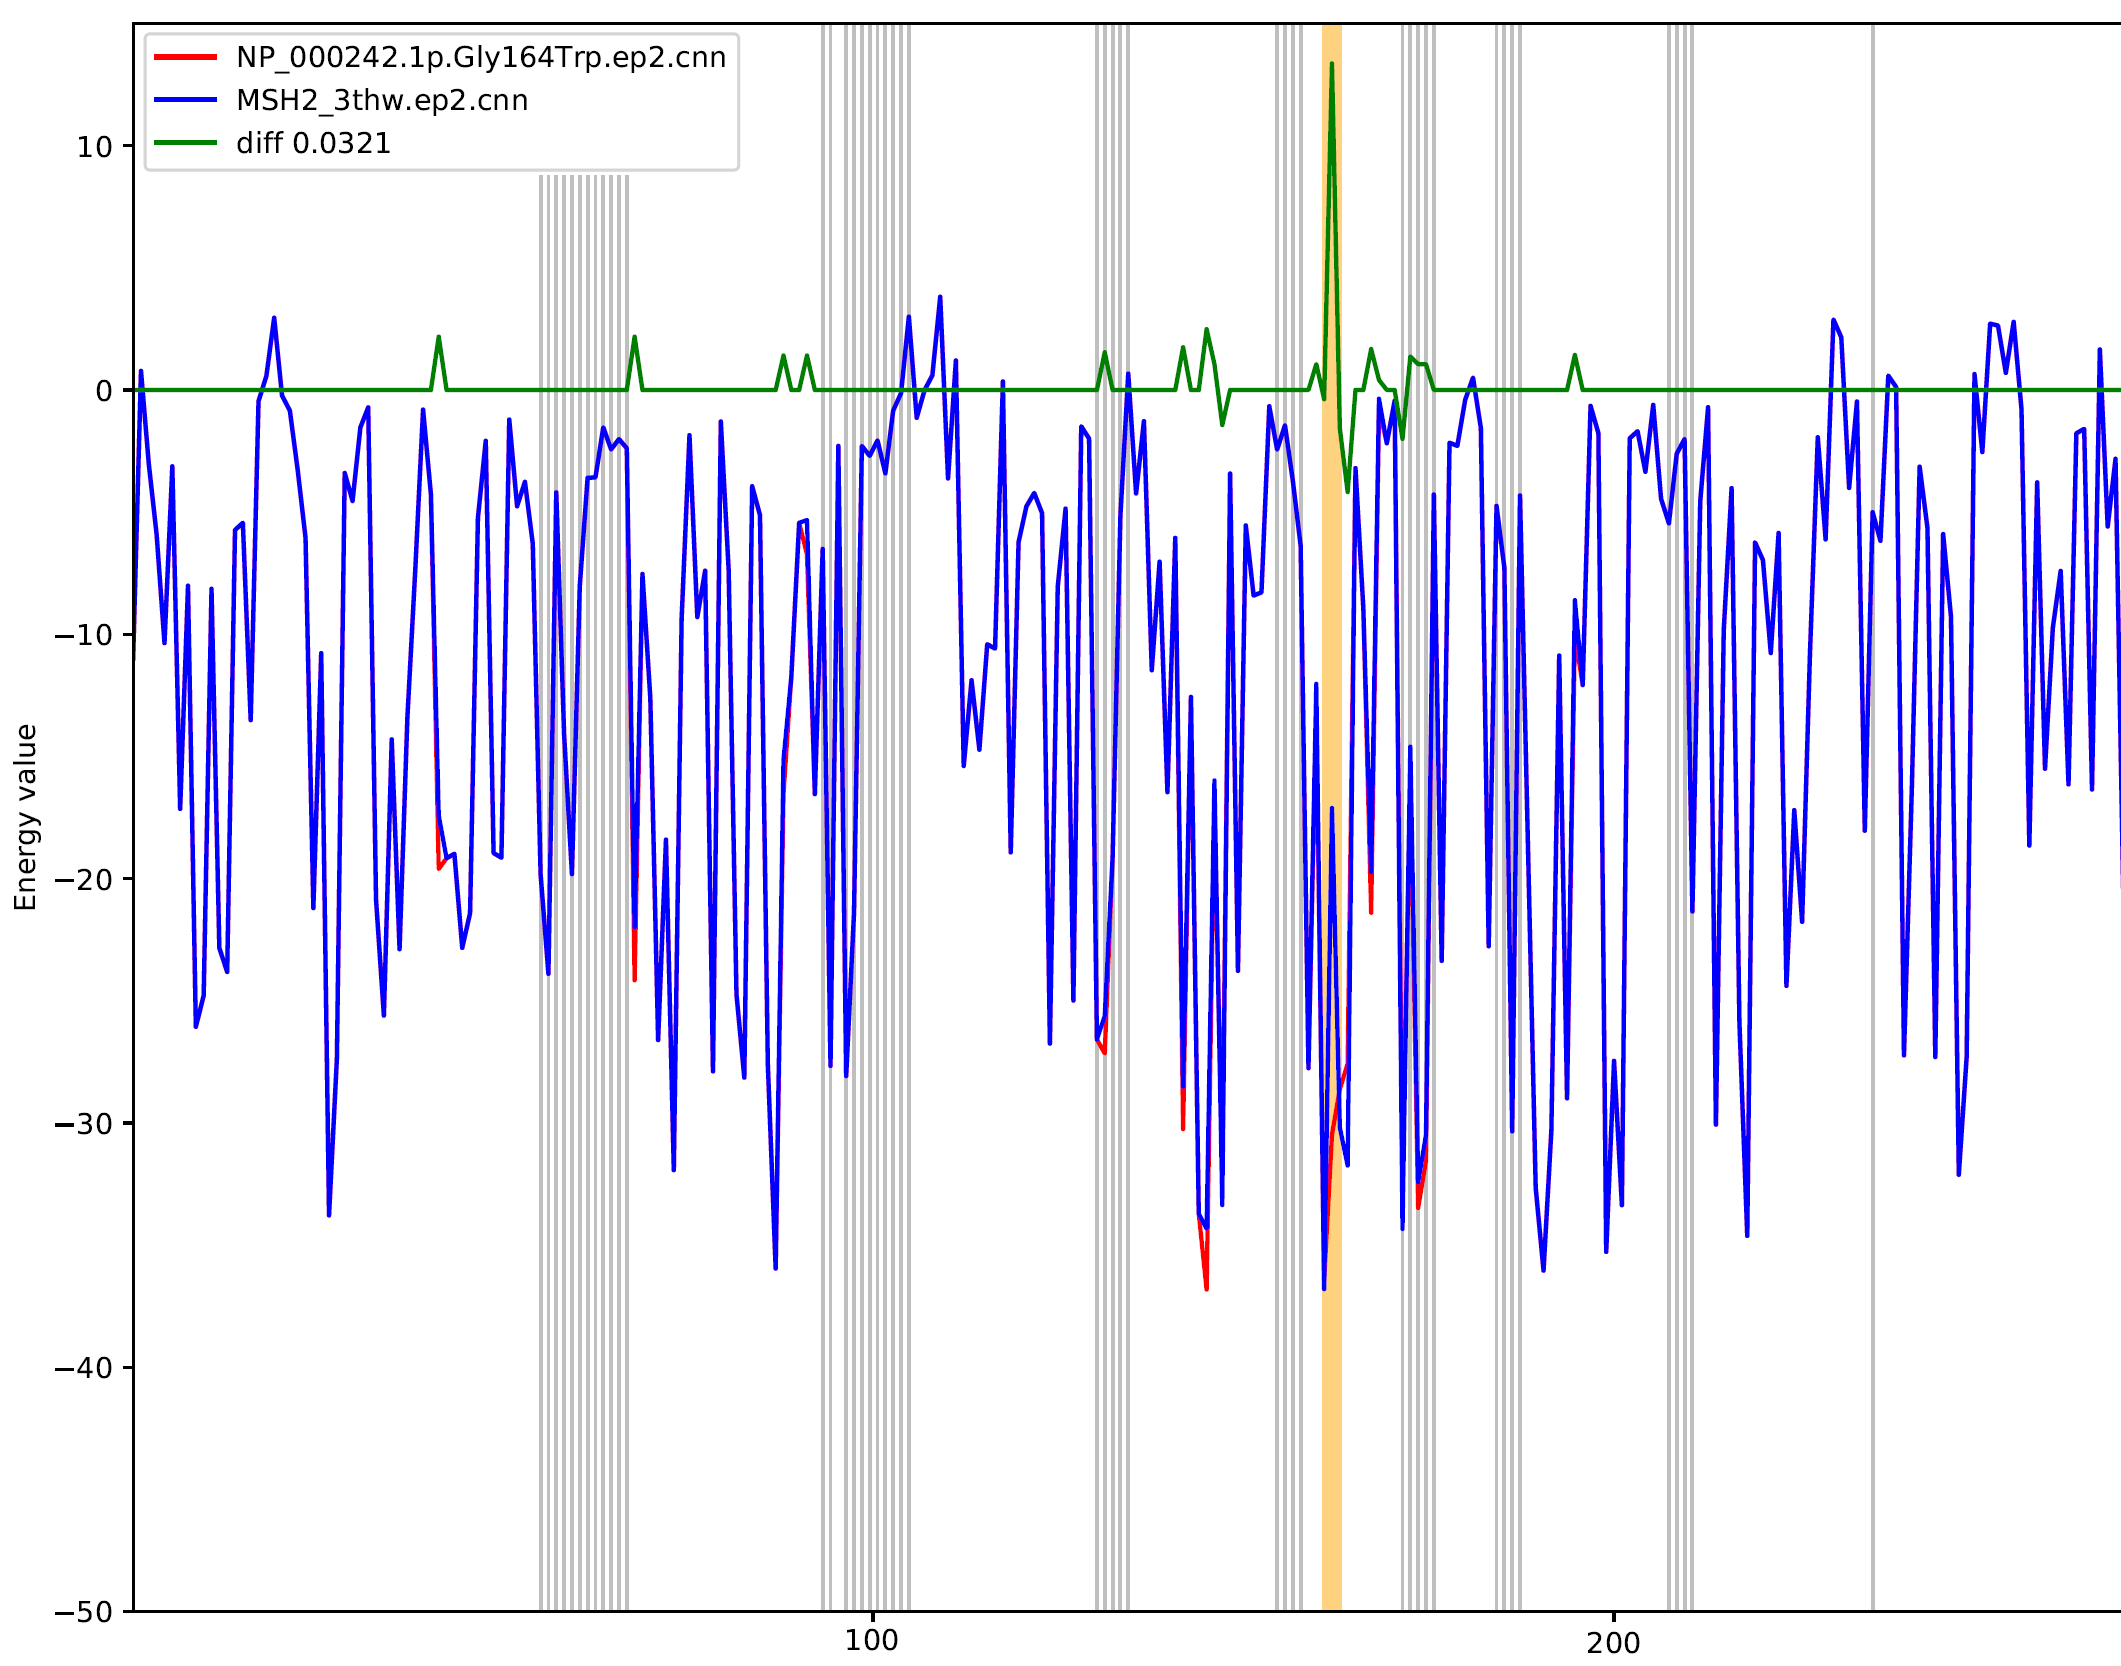
\includegraphics[width=.90\textwidth]{images/comp_plot_Gly164Trp.png}
    \caption{Ausschnitt aus dem Protein MSH2 mit gutartigem \ac{SNP} an Position 169 und mit pathogenen \ac{SNP} an Position 164. Auf der Abszisse ist die Aminosäureposition und auf der Ordinate sind die Energiewerte aufgetragen. Die Referenzsequenz ist blau, die mutierte Sequenz rot und die Differenz der beiden Sequenzen grün dargestellt. Die Position des \ac{SNP}s ist gelb markiert. Die gesamte Energiedifferenz über alle Aminosäuren ist in der Legende hinter \emph{diff} angegeben.} 
    \label{fig:comp_plot_MSH2}
\end{figure}

So ist an der Position des \ac{SNP}s, sowohl im oberen als auch im unterem Bild eine Veränderung des Energieniveaus zu erkennen. Im oberen Bild wurde ein gutartiger \ac{SNP} geplottet, zu sehen ist eine Substitution von Isoleucin nach Valin an Position 169, das Energieniveau verändert sich um 2,5 Einheiten. 

Im unteren Bild wurde ein pathogener \ac{SNP} geplottet, zu sehen ist hier eine Substitution von Glycin nach Tryptophan an Position 164, das Energieniveau verändert sich um 12,8 Einheiten. 

Zudem wurden nicht nur Veränderungen unmittelbar am \ac{SNP} festgestellt, sondern auch einige nicht ganz so starke Veränderungen an verschiedenen anderen Aminosäuren im Protein, diese Veränderungen treten oft an den vorher berechneten Kontakten der Aminosäure auf. Generell lässt sich sagen, dass es im gesamten Protein zu energetischen Veränderungen kam.

\begin{figure}
    \centering
    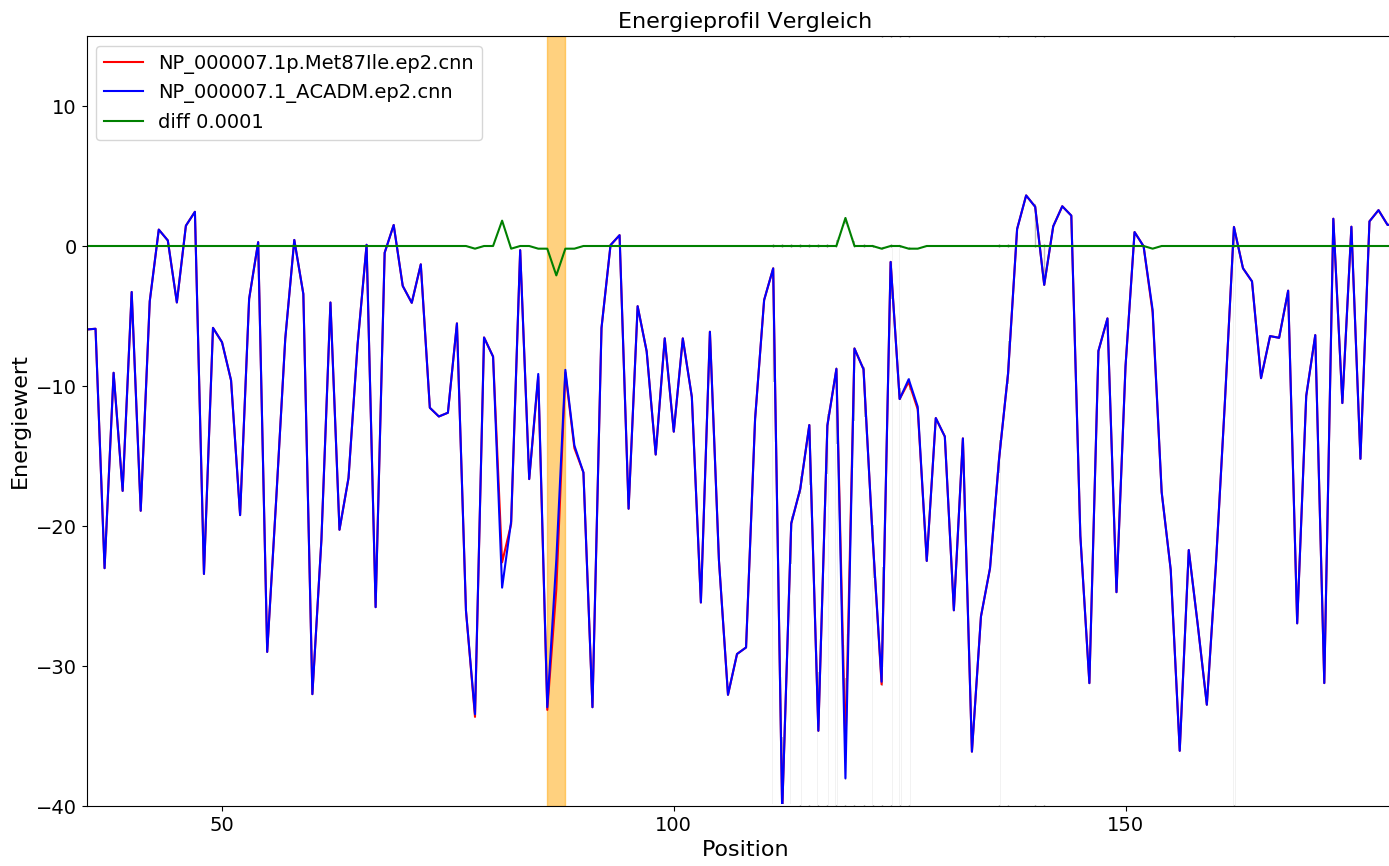
\includegraphics[width=.95\textwidth]{images/comp_plot_ACADM_Met87Ile.png}
    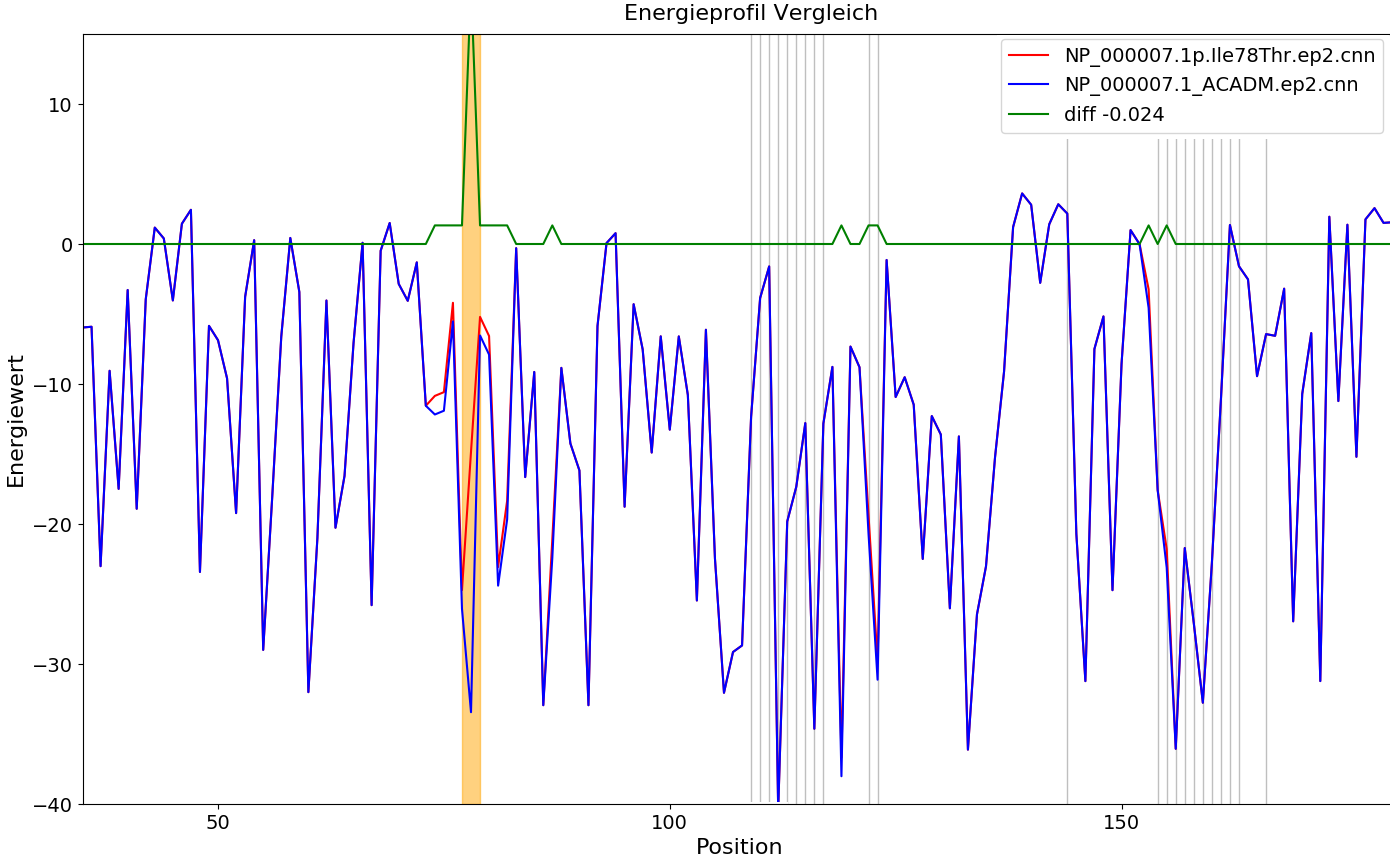
\includegraphics[width=.95\textwidth]{images/comp_plot_ACADM_Ile78Thr.png}
    \caption{Ausschnitt aus dem Protein ACADM mit gutartigem \ac{SNP} an Position 78 und mit pathogenen \ac{SNP} an Position 87. Auf der Abszisse ist die Aminosäureposition und auf der Ordinate sind die Energiewerte aufgetragen. Die Referenzsequenz ist blau, die mutierte Sequenz rot und die Differenz der beiden Sequenzen grün dargestellt. Die Position des \ac{SNP}s ist gelb markiert. Die gesamte Energiedifferenz über alle Aminosäuren ist in der Legende hinter \emph{diff} angegeben.}
    \label{fig:comp_plot_ACADM}
\end{figure}

Als weiteres Beispiel dient die \ac{Abb} \ref{fig:comp_plot_ACADM}, hier ist der Anfang des globulären Proteins \texttt{ACADM} dargestellt. Diese Abbildung ist genau wie \ac{Abb} \ref{fig:comp_plot_MSH2} aufgebaut, so sind die fortlaufenden Aminosäuren auf der Abszisse und die Energiewerte befinden sich auf der Ordinate. Im oberen Bild der \ac{Abb} \ref{fig:comp_plot_ACADM} ist der \ac{SNP} Met87Ile eingetragen, der eine Substitution von Methionin nach Isoleucin an der Position 87 im Protein zeigt. Dies verringert den Energiewert an dieser Stelle um etwa 1,5, an den Kontakten und generell in der gesamtem Sequenz, wurden nur sehr kleine Veränderungen festgestellt.

Im unteren Bild der \ac{Abb} \ref{fig:comp_plot_ACADM}, ist eine Substitution an Position 78 von Isoleucin auf Threonin zu erkennen. Der Energiewert an dieser Position wurde um etwa 15 erhöht. Zwei Positionen vor und hinter dem \ac{SNP} sieht man ebenfalls eine Erhöhung des Energieniveau um 1,5.

Die restlichen Plots, also jene welche für die Erstellung der Tabellen \ref{tab:snps_memb} und \ref{tab:snps_glob} notwendig waren, befinden sich im Online Anhang dieser Arbeit.



\newpage
\section{Auswertung}
\label{sec:snp_auswertung}
Der Datensatz aus Kapitel \ref{sec:auswertung_eps} enthielt 85 \ac{SNP}s, da jedoch nicht alle SNPs innerhalb der aufgeklärten Struktur lagen, bestand der Datensatz am Ende aus 55 \ac{SNP}s, aus den Genen \texttt{MSH2, CFTR, ACADM, PMS2, SLC2A1} und \texttt{SDHB}. Nun wurde nach Kriterien gesucht, um diese SNPs zu trennen. 

\begin{table}[H]
    \centering
    \caption{Dargestellt sind alle alpha helicalen Membranproteine mit \ac{SNP}s, die auf den aufgeklärten Strukturen liegen. Die \texttt{SNP} Zeile gibt an welche Aminosäure an welcher Position ausgetauscht wurde. Die \texttt{ClinVar} Zeile zeigt die offizielle ClinVar Annotation des jeweiligen \ac{SNP}s an. Die \texttt{snp\_diff} Zeile zeigt die Differenz zwischen Mutation und Referenz. Die \texttt{snp\_diff\_amount} Zeile gibt die absolute Differenz zwischen Mutation und Referenz. Die \texttt{total\_diff} Zeile zeigt die Totale Energiedifferenz über die gesamte Polypeptidkette. Die \texttt{total\_contact\_diff} Zeile gibt die Energiedifferenz über alle Kontakte an. Pathogene \ac{SNP}s sind rot und gutartige \ac{SNP}s sind grün markiert, die Tabelle ist aufsteigend nach der blauen Kopfzeile sortiert.}
    \label{tab:snps_memb}
    \resizebox{\linewidth}{!}{%
    \begin{tabular}{llllll}
    \hline
    \multicolumn{1}{|l|}{SNP} & \multicolumn{1}{l|}{ClinVar} & \multicolumn{1}{l|}{\cellcolor[HTML]{BBDAFF}snp\_diff} & \multicolumn{1}{l|}{snp\_diff\_amount} & \multicolumn{1}{l|}{total\_diff} & \multicolumn{1}{l|}{total\_contact\_diff} \\ \hline
    \rowcolor[HTML]{FFCCC9} 
    Cys192Arg & pathogenic & -28,58 & 28,58 & 63,35 & 48,27 \\
    \rowcolor[HTML]{FFCCC9} 
    Cys196Tyr & pathogenic & -13,57 & 13,57 & 37,29 & 26,18 \\
    \rowcolor[HTML]{FFCCC9} 
    Ile127Ser & pathogenic & -7,07 & 7,07 & 15,16 & 11,25 \\
    \rowcolor[HTML]{FFCCC9} 
    Val140Phe & pathogenic & -2,53 & 2,53 & 15,71 & 5,36 \\
    \rowcolor[HTML]{9AFF99} 
    Gly53Glu & benign & -2,43 & 2,43 & 7,27 & 4,86 \\
    \rowcolor[HTML]{9AFF99} 
    His57Arg & benign & -1,21 & 1,21 & 4,85 & 2,08 \\
    \rowcolor[HTML]{9AFF99} 
    Ser163Pro & benign & -0,90 & 0,90 & 46,12 & 7,72 \\
    \rowcolor[HTML]{FFCCC9} 
    Pro197Arg & pathogenic & -0,39 & 0,39 & 3,20 & 0,62 \\
    \rowcolor[HTML]{FFCCC9} 
    Arg46Gln & pathogenic & 1,06 & 1,06 & 4,53 & 2,01 \\
    \rowcolor[HTML]{FFCCC9} 
    Arg230His & pathogenic & 2,43 & 2,43 & 7,28 & 5,37 \\
    \rowcolor[HTML]{FFCCC9} 
    Arg242His & pathogenic & 3,54 & 3,54 & 14,10 & 7,39 \\
    \rowcolor[HTML]{FFCCC9} 
    Trp200Cys & pathogenic & 8,74 & 8,74 & 69,42 & 19,57 \\
    \rowcolor[HTML]{FFCCC9} 
    Arg242Cys & pathogenic & 20,53 & 20,53 & 41,07 & 33,17
    \end{tabular}}
\end{table}

% Please add the following required packages to your document preamble:
% \usepackage[table,xcdraw]{xcolor}
% If you use beamer only pass "xcolor=table" option, i.e. \documentclass[xcolor=table]{beamer}
\begin{table}[]
    \centering
    \caption{Zu sehen sind alle globulären Proteine, mit ihren jeweiligen \ac{SNP}s. Die Tabelle ist genau wie \ref{tab:snps_memb} aufgebaut, mit dem Zusatz, dass \ac{SNP}s welche widersprüchliche Annotationen haben grau und \ac{SNP}s mit nur einem Autor hell grün dargestellt sind.}
    \label{tab:snps_glob}
    \resizebox{\linewidth}{!}{%
    \begin{tabular}{llllll}
        \hline
        \multicolumn{1}{|l|}{SNP} & \multicolumn{1}{l|}{ClinVar} & \multicolumn{1}{l|}{snp\_diff} & \multicolumn{1}{l|}{\cellcolor[HTML]{BBDAFF}snp\_diff\_amount} & \multicolumn{1}{l|}{total\_diff} & \multicolumn{1}{l|}{total\_contact\_diff} \\ \hline
        \rowcolor[HTML]{FFCCC9} 
        Gly164Arg & pathogenic & -0,27 & 0,27 & 265,91 & 46,75 \\
        \rowcolor[HTML]{FFCCC9} 
        Leu84Phe & pathogenic & 0,78 & 0,78 & 18,38 & 5,41 \\
        \rowcolor[HTML]{FFCCC9} 
        Gly162Arg & pathogenic & -0,81 & 0,81 & 71,01 & 11,34 \\
        \rowcolor[HTML]{FFCCC9} 
        Gly267Arg & pathogenic & -0,93 & 0,93 & 5,39 & 4,12 \\
        \rowcolor[HTML]{9AFF99} 
        Gln629Arg & benign & 1,05 & 1,05 & 2,11 & 2,11 \\
        \rowcolor[HTML]{9AFF99} 
        Leu390Phe & benign & 1,36 & 1,36 & 51,55 & 4,10 \\
        \rowcolor[HTML]{FFCCC9} 
        Arg359Ser & pathogenic & 1,40 & 1,40 & 2,79 & 2,58 \\
        \rowcolor[HTML]{FFCCC9} 
        Pro349Arg & pathogenic & 1,89 & 1,89 & 147,84 & 15,61 \\
        \rowcolor[HTML]{9AFF99} 
        Met87Ile & benign & 2,10 & 2,10 & 7,82 & 5,44 \\
        \rowcolor[HTML]{9AFF99} 
        Ile145Met & benign & -2,48 & 2,48 & 10,41 & 5,82 \\
        \rowcolor[HTML]{9AFF99} 
        Ala834Thr & benign & -2,74 & 2,74 & 5,47 & 5,47 \\
        \rowcolor[HTML]{9AFF99} 
        Ile169Val & benign & -3,13 & 3,13 & 6,26 & 5,64 \\
        \rowcolor[HTML]{9AFF99} 
        Asn596Ser & benign & 3,25 & 3,25 & 6,50 & 6,23 \\
        \rowcolor[HTML]{9AFF99} 
        Gly322Asp & benign & -3,35 & 3,35 & 13,18 & 9,00 \\
        \rowcolor[HTML]{FFCCC9} 
        Arg294Thr & pathogenic & 3,37 & 3,37 & 9,21 & 6,44 \\
        \rowcolor[HTML]{9AFF99} 
        Asn127Ser & benign & 3,52 & 3,52 & 7,04 & 6,23 \\
        \rowcolor[HTML]{9AFF99} 
        Gln419Lys & benign & -3,54 & 3,54 & 7,08 & 7,08 \\
        \rowcolor[HTML]{FFCCC9} 
        Gly195Arg & pathogenic & -3,68 & 3,68 & 26,82 & 23,39 \\
        \rowcolor[HTML]{9AFF99} 
        Cys159Trp & benign & -3,85 & 3,85 & 49,76 & 28,47 \\
        \rowcolor[HTML]{9AFF99} 
        Thr564Ala & benign & 4,11 & 4,11 & 8,21 & 8,21 \\
        \rowcolor[HTML]{9AFF99} 
        Arg106Lys & benign & -5,74 & 5,74 & 11,48 & 11,48 \\
        \rowcolor[HTML]{FFCCC9} 
        Cys333Tyr & pathogenic & -7,13 & 7,13 & 152,62 & 12,20 \\
        \rowcolor[HTML]{FFCCC9} 
        Asp266Gly & pathogenic & 7,21 & 7,21 & 16,82 & 11,79 \\
        \rowcolor[HTML]{FFCCC9} 
        Tyr67His & pathogenic & -8,19 & 8,19 & 16,38 & 14,84 \\
        \rowcolor[HTML]{FFCCC9} 
        Gly338Glu & pathogenic & -8,26 & 8,26 & 105,26 & 22,93 \\
        \rowcolor[HTML]{EFEFEF} 
        Ala272Val & benign & 8,39 & 8,39 & 51,22 & 17,28 \\
        \rowcolor[HTML]{CBFFCB} 
        Glu198Gly & benign & 10,58 & 10,58 & 21,15 & 17,57 \\
        \rowcolor[HTML]{EFEFEF} 
        Asp167His & benign & 11,05 & 11,05 & 144,93 & 28,80 \\
        \rowcolor[HTML]{FFCCC9} 
        Arg53Cys & pathogenic & 12,82 & 12,82 & 26,12 & 26,12 \\
        \rowcolor[HTML]{FFCCC9} 
        Gly164Trp & pathogenic & 13,36 & 13,36 & 108,76 & 40,34 \\
        \rowcolor[HTML]{FFCCC9} 
        Pro349Leu & pathogenic & 13,42 & 13,42 & 86,91 & 32,69 \\
        \rowcolor[HTML]{FFCCC9} 
        Ser245Leu & pathogenic & 15,36 & 15,36 & 30,73 & 28,08 \\
        \rowcolor[HTML]{FFCCC9} 
        Thr121Ile & pathogenic & 15,94 & 15,94 & 31,26 & 26,40 \\
        \rowcolor[HTML]{FFCCC9} 
        Leu187Arg & pathogenic & -17,93 & 17,93 & 168,07 & 33,17 \\
        \rowcolor[HTML]{FFCCC9} 
        Ile78Thr & pathogenic & -18,60 & 18,60 & 37,20 & 34,54 \\
        \rowcolor[HTML]{FFCCC9} 
        Leu187Pro & pathogenic & -19,39 & 19,39 & 567,70 & 32,50 \\
        \rowcolor[HTML]{FFCCC9} 
        Leu310Pro & pathogenic & -20,13 & 20,13 & 97,78 & 35,09 \\
        \rowcolor[HTML]{FFCCC9} 
        Val163Gly & pathogenic & -21,48 & 21,48 & 49,06 & 40,89 \\
        \rowcolor[HTML]{FFCCC9} 
        Cys199Arg & pathogenic & -21,49 & 21,49 & 106,18 & 36,86 \\
        \rowcolor[HTML]{FFCCC9} 
        Val200Asp & pathogenic & -22,11 & 22,11 & 44,22 & 36,02 \\
        \rowcolor[HTML]{FFCCC9} 
        Val163Asp & pathogenic & -27,66 & 27,66 & 55,33 & 48,98
    \end{tabular}}
\end{table}

Um eine bestmögliche Klassifizierung der \ac{SNP}s zu erhalten, wurden die \ac{SNP}s nach Membran und globulärer Assoziation getrennt. So enthielt die Tabelle \ref{tab:snps_memb} mit den Membranproteinen 13 \ac{SNP}s, welche eindeutig nach ihrer Differenz am \ac{SNP} klassifiziert werden konnten. Indem die untere Grenze bei -2,5 und die obere Grenze bei -0,3 fest gelegtwurde. Somit sind alle \ac{SNP}s pathogen, wenn sie unter oder über dieser Grenze liegen.

Damit errechnete sich ein MCC Wert von 1,0, da die Anzahl der \emph{False Positves} und \emph{False Negatives} bei 0 lag.

Bei der Tabelle \ref{tab:snps_glob} mit den globulären Proteinen, wurde nach der absoluten Energiedifferenz am \ac{SNP} sortiert und klassifiziert. Dies hat einen MCC Wert von 0,8 geliefert, wenn die untere Grenze auf 2 und die obere Grenze auf 7 festgelegt wird. Zusätzlich wurde noch nach drei anderen Kriterien klassifiziert, siehe Tabelle \ref{tab:mcc_table}. So wurde ein MCC von 0,65 ermittelt, wenn die \ac{SNP}s nach der Differenz zwischen Mutation und Referenz am \ac{SNP} sortiert wurden, als untere Grenze wurde hier -6 ermittelt und als obere Grenze 4,5. Wenn die \ac{SNP}s nach der totalen Energiedifferenz über die gesamte Polypeptidkette sortiert werden, kommt man auf einen MCC von 0,77, wenn man die untere Grenze auf 0 und die obere Grenze auf 14 setzt. Wenn man die \ac{SNP}s nach der Energiedifferenz über alle Kontakte sortiert, kommt man auf einen MCC von 0,75. Hierbei wurde die untere Grenze auf 0 und die obere Grenze auf 11,5 festgelegt.

\begin{table}[]
    \centering
    \caption{Dargestellt ist die jeweilige Anzahl an tp = \emph{true positives}, fp = \emph{false postives}, tn = \emph{true negatives} und fn = \emph{false negatives}, für die Sortierung und Klassifizierung der \ac{SNP} Daten. Am Ende der Tabelle steht der jeweilige \acf{MCC}. Die \texttt{snp\_diff} Zeile zeigt die Differenz zwischen Mutation und Referenz. Die \texttt{snp\_diff\_amount} Zeile gibt die absolute Differenz zwischen Mutation und Referenz. Die \texttt{total\_diff} Zeile zeigt die Totale Energiedifferenz über die gesamte Polypeptidkette. Die \texttt{total\_contact\_diff} Zeile gibt die Energiedifferenz über alle Kontakte an.}
    \label{tab:mcc_table}
    \begin{tabular}{l|l|l|l|l|}
        \cline{2-5}
         & snp\_diff & snp\_diff\_amount & total\_diff & total\_contact\_diff \\ \hline
        \multicolumn{1}{|l|}{TP} & 17 & 21 & 22 & 20 \\ \hline
        \multicolumn{1}{|l|}{TN} & 13 & 13 & 11 & 12 \\ \hline
        \multicolumn{1}{|l|}{FP} & 0 & 0 & 1 & 0 \\ \hline
        \multicolumn{1}{|l|}{FN} & 8 & 4 & 3 & 5 \\ \hline
        \multicolumn{1}{|l|}{MCC} & \cellcolor[HTML]{FFFFC7}0,65 & \cellcolor[HTML]{9AFF99}0,80 & \cellcolor[HTML]{CBFFCB}0,77 & \cellcolor[HTML]{E2FFE2}0,75 \\ \hline
    \end{tabular}
\end{table}



%\newpage
\section{Ramachandran Plot Ergebnis}
Bedingt durch die Tatsache, dass alle in dieser Arbeit \ref{sec:konst} gefilterten \ac{Pfams} auch eine aufgeklärte Struktur besitzen lies sich nun jede \ac{Pfam} in einen Ramachandran Plot darstellen, siehe z.B. \ac{Abb} \ref{fig:ramachandran_PF01287}. Auf dieser Abbildung, sind die Cluster Winkel der Beta Faltblätter oben links bei -150 $\phi$ und -100 $\psi$ zu erkennen. Zudem sind die rechts drehenden Alpha Helices bei -25 $\phi$ und -75 $\psi$ zu erkennen. Bei genauerer Betrachtung sind auch die links drehenden Alpha Helices, bei +/-10\ $\phi$ und 100 $\psi$ als Anhäufung, zu sehen. So wie man es auch in \ac{Abb} \ref{fig:ramaplot} gesehen hat. Der \ac{SNP} in der Aminosäuresequenz \texttt{1bkb} äußert sich in einer Winkelveränderung, diese ist als roter Punkt dargestellt.

\begin{figure}
    \centering
    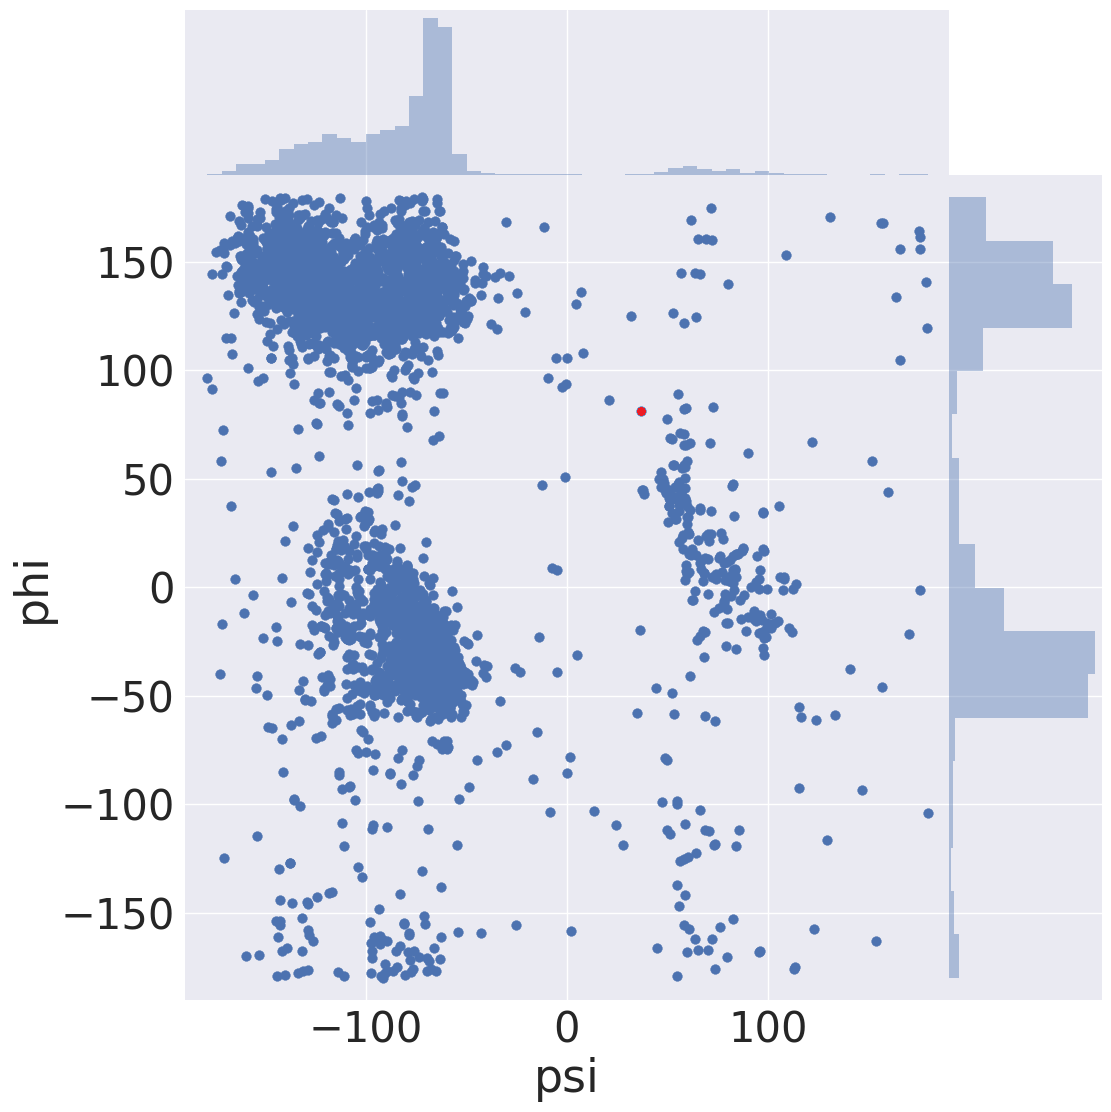
\includegraphics[width=.90\textwidth]{images/ramachandranplot_PF01287.png}
    \caption{Ramachandran Plot der Pfam PF01287. Auf der Abszisse sind die PSI und auf der Ordinate sind die PHI Winkel aufgetragen. Das Histogramm auf der Abszisse zeigt das Vorkommen der PSI Winkel, das Histogramm auf der Ordinate das Vorkommen der PHI Winkel. Der \ac{SNP} in der Aminosäuresequenz \texttt{1bkb} ist als roter Punkt dargestellt.}
    \label{fig:ramachandran_PF01287}
\end{figure}


